\chapter{Statistical inference}
\label{chap:hgg_stats}

\section{Introduction}
The statistical methodology used to extract the results follows the procedure developed by the ATLAS and CMS collaborations, documented in Ref.~\cite{Khachatryan:2014jba}. 

\subsection{Construction of the per-category likelihood}\label{sec:category_likelihood}
A simultaneous binned maximum likelihood fit is performed to the $m_{\gamma\gamma}$ distributions of all analysis categories. This requires the construction of a likelihood function for each analysis category, $k$, of the form,

\begin{equation}\label{eq:category_likelihood}
\begin{split}
    L_k({\rm{data}}\,|\,\mu^{i,\gamma\gamma},m_H,\vec{\theta}_s,\vec{\theta}_b) = \\
    \prod^{N_{\rm{bins}}}_{X} {\rm{Poisson}} \Big( N_{k,X}^{\rm{data}} \, \Big| \, \Big[ \sum_{i} S_{k,X}^{i,\gamma\gamma}(\mu^{i,\gamma\gamma},m_H,\vec{\theta}_s)\Big] + B_{k,X}(\vec{\theta}_b) \Big) \times \mathcal{C}(\vec{\theta}_s,\vec{\theta}_b),        
\end{split}
\end{equation}

\noindent
where the index, $X$, runs over bins in the $m_{\gamma\gamma}$ distribution in the range $100<m_{\gamma\gamma}<180$~GeV with a bin width of 250~MeV (CHECK!); this choice is sufficiently small compared to the diphoton mass resolution to ensure that a negligible amount of information is lost. The likelihood itself is a function of the signal parameters, $\mu^{i,\gamma\gamma}$, the Higgs boson mass, $m_H$, and nuisance parameters, $\vec{\theta}$~=~$\{\vec{\theta}_s,\vec{\theta}_b\}$, which account for systematic uncertainties in the signal and background estimates. The nuisance parameters are grouped according to their effect, as shown in equation \ref{eq:systematics_grouping},

\begin{equation}\label{eq:systematics_grouping}
    \big\{\vec{\theta}_s,\vec{\theta}_b\big\} = \big\{ \vec{\theta}^{\,\rm{th}}_{s}, \vec{\theta}^{\,\epsilon,{\rm{th}}}_{s}, \vec{\theta}^{\,\epsilon,{\rm{exp}}}_{s}, \vec{\theta}^{\,\rm{shape}}_{s}, \vec{\theta}^{\,\rm{lumi}}_{s}, \vec{\theta}^{\,\rm{shape}}_{b}, \vec{\theta}^{\,\rm{discrete}}_{b}  \big\},
\end{equation}

\noindent
where $\vec{\theta}^{\,\rm{th}}_{s}$ are the uncertainties in the SM prediction of the cross sections times branching ratio, $[\sigma^i \cdot \mathcal{B}^{\gamma\gamma}]_{\rm{SM}}$. The $\vec{\theta}^{\,\epsilon,{\rm{th}}}_{s}$ and $\vec{\theta}^{\,\epsilon,{\rm{exp}}}_{s}$ terms correspond to systematic uncertainties in the efficiency times acceptance of the final analysis categories, originating from theoretical and experimental sources respectively. Nuisance parameters affecting the shape of the analytic signal model, described in more detail in section \ref{sec:sig_modelling}, are labelled by $\vec{\theta}^{\,\rm{shape}}_{s}$. The uncertainties in the luminosity are referred to as $\vec{\theta}^{\,\rm{lumi}}_{s}$; these affect only the signal estimate as the background estimate is derived directly from data. Finally, the background model shape parameters are labelled as $\vec{\theta}^{\,\rm{shape}}_{b}$, whilst the discrete nuisance parameters corresponding to the uncertainty in the choice of background function are labelled as $\vec{\theta}^{\,\rm{discrete}}_{b}$. More detail concerning the individual sources of the systematic uncertainties is provided in section \ref{sec:systematics}.

In the poisson term of the likelihood, $N_{k,X}^{\rm{data}}$, corresponds to the number of data events in bin $X$ of category $k$, and $S_{k,X}^{i,\gamma\gamma}$ and $B_{k,X}$ are the signal and background estimates in the same bin. The index, $i$, labels the particular \textit{signal process}, which in this analysis corresponds to the STXS stage 1.2 bins (i.e. the sum in equation \ref{eq:category_likelihood} iterates over all STXS bins). Equation \ref{eq:signal_yield} shows the total signal yield for process, $i$, in analysis category, $k$, integrated over all $m_{\gamma\gamma}$ bins,

\begin{equation}\label{eq:signal_yield}
    S_k^{i,\gamma\gamma} = \mu^{i,\gamma\gamma} \times \big[\sigma^i \cdot \mathcal{B}^{\gamma\gamma} \big]_{\rm{SM}}(m_H,\vec{\theta}^{\,\rm{th}}_{s}) \times \epsilon^{i,\gamma\gamma}_k(m_H,\vec{\theta}^{\,\epsilon,{\rm{th}}}_{s}, \vec{\theta}^{\,\epsilon,{\rm{exp}}}_{s}) \times \mathcal{L}(\vec{\theta}^{\,\rm{lumi}}_{s}).
\end{equation}

\noindent
Here $[\sigma^i \cdot \mathcal{B}^{\gamma\gamma}]_{\rm{SM}}$ is the SM prediction for the cross section times branching ratio for process $i$, listed in Tables XX-YY for $m_H$~=~125.0~GeV. The product of the detector efficiency and the analysis acceptance is represented by $\epsilon^{i,\gamma\gamma}_k$, which effectively encodes the fraction of the total yield of process, $i$, which lands in analysis category, $k$, and the luminosity estimate is represented by $\mathcal{L}$. The signal parameters, $\mu^{i,\gamma\gamma}$, define the \textit{parameters of interest}. For example, when measuring cross sections in the STXS framework,

\begin{equation}\label{eq:mu_stxs}
    \mu^{i,\gamma\gamma} = \frac{\big[\sigma^i \cdot \mathcal{B}^{\gamma\gamma} \big]_{\rm{obs}}\hfill}{\big[\sigma^i \cdot \mathcal{B}^{\gamma\gamma} \big]_{\rm{SM}}(m_H,\vec{\theta}^{\,\rm{th}}_{s})}.
\end{equation}

\noindent
In this signal parametrisation, the theory systematic uncertainties, $\vec{\theta}^{\,\rm{th}}_{s}$, in the denominator of equation \ref{eq:mu_stxs} cancel out the same terms in equation \ref{eq:signal_yield}. As a result, $\vec{\theta}^{\,\rm{th}}_{s}$, do not enter the cross section measurements, but are instead attributed to the uncertainty in the SM predictions (see grey bands of Figure \ref{fig:stxs_maximal}). This property of the measurements has the added benefit that they remain useful in the long-term, as they can accommodate future advances in the SM theoretical predictions.

Other signal parametrisations are considered. The per-production mode signal strength parametrisation defines four POIs: $\mu_{\rm{ggH}}$, $\mu_{\rm{VBF}}$, $\mu_{\rm{VH}}$ and $\mu_{\rm{top}}$, which act as global scaling factors for the respective Higgs boson production modes. The $\kappa$-framework~\cite{Heinemeyer:2013tqa} replaces $\mu^{i,\gamma\gamma}$ with functions of Higgs boson coupling modifiers ($\kappa$-parameters), $\mu^{i,\gamma\gamma}(\vec{\kappa})$, where the form of the function depends on the signal process, $i$ (see section \ref{sec:results_kappa})\footnote{Looking ahead to Section \ref{chap:eft}, here the signal yields are parametrised in an EFT framework, $\mu^{i,\gamma\gamma}(c_j)$, so that the same statistical procedure can be used to extract constraints on EFT parameters, $c_j$.}. In such \textit{interpretations}, there is no cancellation of $\vec{\theta}^{\,\rm{th}}_{s}$, meaning these nuisance parameters are directly folded into the measurements. In general, we can write $\mu^{i,\gamma\gamma}$ as a function of some set of parameters of interest, $\vec{\alpha}$,

\begin{equation}
    \mu^{i,\gamma\gamma} \equiv \mu^{i,\gamma\gamma}(\vec{\alpha}).
\end{equation}

To determine $S_{k,X}^{i,\gamma\gamma}$ (i.e the fraction of $S_k^{i,\gamma\gamma}$ that falls in bin $X$ of the $m_{\gamma\gamma}$ distribution), it is necessary to model the functional form of the signal peak in the diphoton invariant mass distribution. Analytic models are constructed for each process, $i$, in each reconstructed analysis category, $k$. More information regarding the signal modelling is provided in section \ref{sec:sig_modelling}.

The background model is derived directly from the observed diphoton mass distribution in data. Described in more detail in section \ref{sec:bkg_modeling}, the form of the analytic model in each analysis category is treated as a discrete nuisance parameter in the fit, with options coming from a number of different smoothly-falling functions. The background estimate, $B_{k,X}$, is inferred from the analytic background model.

Finally, the constraint term in the likelihood, $\mathcal{C}$, applies a penalty for deviations from the expected values of the signal nuisance parameters, $\vec{\theta}_s$. The form of this penalty depends on the choice of prior probability-density-function (pdf) for a given nuisance; in this analysis all nuisance parameters affecting the signal estimate are associated with a Gaussian or log-normal prior. The background nuisance parameters, $\vec{\theta}_b$, are instead associated with a flat prior, since there is no a-priori knowledge of their values, and therefore changes in their value are not explicitly penalised by the constraint term. However, an additional penalty is included according to the total number of degrees of freedom in the background model function (CHECK!). 

\subsection{Extraction of results}\label{sec:results_extraction}
The total likelihood function is defined as the product over all 80 per-category likelihoods,

\begin{equation}
    L({\rm{data}}\,|\,\vec{\alpha},m_H,\vec{\theta}) = \prod_{k=1}^{80}  L_k({\rm{data}}\,|\,\vec{\alpha},m_H,\vec{\theta}),
\end{equation}

\noindent
where the signal parameters, $\mu^{i,\gamma\gamma}$, have been expressed in terms of the general parameters of interest, $\vec{\alpha}$, and $\vec{\theta}$~=~$\{\vec{\theta}_s,\vec{\theta}_b\}$. In all fits, the Higgs boson mass, $m_H$, is fixed to its most precisely measured value of 125.38~GeV~\cite{Sirunyan:2020xwk}. This ensures all measurements are reported with respect to the theoretical predictions consistent with the best available knowledge of $m_H$. Ultimately, the fixing of the Higgs boson mass means the dependence of the likelihood on $m_H$ is dropped.

In practice, the fit is performed by minimising the value of $-2 \ln L({\rm{data}}\,|\,\vec{\alpha},\vec{\theta})$. This is done numerically using the RooFit software package~\cite{Verkerke:2003ir}. The values of the parameters of interest which minimise this quantity are described as the ``best-fit" values, and are labelled as the point in the parameter space, $\hat{\vec{\alpha}}$. The values of the nuisance parameters at this point, $\hat{\vec{\theta}}$, are referred to as the unconditional maximum likelihood estimates of $\vec{\theta}$. 

To calculate the confidence intervals for the parameters of interest, a profile likelihood test statistic, $q(\vec{\alpha})$ is constructed as shown in equation \ref{eq:test_statistic},

\begin{equation}\label{eq:test_statistic}
    q(\vec{\alpha}) = -2 \ln \Bigg( \frac{L({\rm{data}}\,|\,\vec{\alpha},\hat{\vec{\theta}}_{\vec{\alpha}})}{L({\rm{data}}\,|\,\hat{\vec{\alpha}},\hat{\vec{\theta}})} \Bigg).
\end{equation}

\noindent
The quantity $\hat{\vec{\theta}}_{\vec{\alpha}}$ corresponds to the conditional maximum likelihood estimates of the nuisance parameters, for fixed values of the parameters of interest, $\vec{\alpha}$. For one-dimensional measurements, such as the signal strength and cross section fits, the 68\% and 95\% confidence intervals are defined by the union of intervals for which $q(\alpha)<0.99$ and $q(\alpha)<3.84$, respectively. In the case where there are multiple parameters of interest in the signal parametrisation, the intervals are determined by treating the other parameters as nuisance parameters i.e. profiling them in the minimisation. In practice, for each parameter of interest, $\alpha$, the minimisation is performed for a discrete set of points, and the full $q(\alpha)$ distribution is determined by interpolating between these points. The number of points is chosen to sufficiently cover the shape of the $q(\alpha)$ distribution.

For two-dimensional measurements, such as those performed in the $\kappa$-framework (see Figure \ref{fig:kappas}), the 68\% and 95\% confidence regions are defined by the set of parameter values for which $q(\alpha_1,\alpha_2)<2.30$ and $q(\alpha_1,\alpha_2)<5.99$, respectively. Again, the full $q(\alpha_1,\alpha_2)$ distribution is determined by performing the numerical minimisation for a discrete grid of parameter points, $(\alpha_1,\alpha_2)$, and interpolating between these values.

In addition to the observed results, it useful to compute the results one would expect to obtain given the SM hypothesis. These so-called \textit{expected results} are determined by replacing the observed data with an Asimov toy dataset, in which all parameters take their SM expected values and all statistical fluctuations are suppressed~\cite{Cowan:2010js}.


\section{Signal modelling}\label{sec:sig_modelling}
The analytic signal model, derived using MC simulated events, is constructed to fit the \mgg spectrum of each STXS stage 1.2 bin in each reconstructed analysis category: $\mathcal{S}^{i,\gamma\gamma}_k(m_{\gamma\gamma};m_H,\vec{\theta}^{\rm{shape}}_s)$. The distribution of events depends on whether the selected vertex (section \ref{sec:vertex_selection}) is correctly identified within 1~cm of the true diphoton vertex. For this reason, the right-vertex (RV) and wrong-vertex (WV) scenarios, defined according to the 1~cm threshold, are considered separately when building the signal shape. The final model is the weighted sum of the RV and WV contributions, where $f_{RV}$ is the fraction of simulated events with the selected vertex within 1~cm of the true vertex, calculated separately for each ($i$,$k$) combination,

\begin{equation}
    \mathcal{S}^{i,\gamma\gamma}_k = f_{RV} \cdot \mathcal{S}^{i,\gamma\gamma}_{k,RV} + (1-f_{RV}) \cdot\mathcal{S}^{i,\gamma\gamma}_{k,WV}.
\end{equation}

To account for the variation in detector performance, the signal models are constructed separately for each data-taking year i.e. using independent MC samples which correspond to the 2016, 2017 and 2018 data-taking conditions respectively. In this approach, the variation in the diphoton mass resolution is incorporated into the model, and year-dependent systematic uncertainties on the signal estimate can be propagated to the final fit. The index, $i$, used in section \ref{sec:category_likelihood}, is effectively extended to label each signal process times year e.g. (ggH 0J high \ptH, 2016). This is such that the efficiency times acceptance factor in equation \ref{eq:signal_yield}, $\epsilon_k^{i,\gamma\gamma}$, is derived separately for each year and the luminosity estimate, $\mathcal{L}$, takes the relevant year-dependent value: 35.9~\fbinv for 2016, 41.5~\fbinv for 2017, and 59.4~\fbinv for 2018. Clearly, the signal parametrisation, $\mu^{i,\gamma\gamma}$, and theory predictions, $[\sigma^i \cdot \mathcal{B}^{\gamma\gamma}]_{\rm{SM}}$, are the same for each year.

Each model, $\mathcal{S}^{i,\gamma\gamma}_{k,V}$, consists of a sum of up to five Gaussians, where $V=\{RV,WV\}$ labels the vertex scenario. The parameters of each Gaussian function, namely the mean, width, and the relative contribution to the total model are extracted by performing a fit to the \mgg spectrum of simulated events. In previous CMS \Hgg analyses, each of these parameters, in addition to $f_{RV}$, were represented by a linear function of $m_H$, where the exact form of these functions was derived by simultaneously fitting simulated events corresponding to three values of $m_H$: 120, 125, and 130~GeV. Using this approach, the final signal model shape was defined as a continuous parametric function of $m_H$. Ultimately, this choice was made since the value of $m_H$ was profiled when extracting the final results, reflecting the lack of knowledge with respect to $m_H$ at the time. 

In this analysis the value of $m_H$ is fixed to 125.38~GeV~\cite{Sirunyan:2020xwk}. Instead, the shape parameters are now defined as constants with respect to $m_H$, and are derived using simulated events with $m_H$~=~125.0~GeV only. This approach relies on the perfectly valid assumption that there is little variation in the shape when moving from 125.0 to 125.38~GeV. 

The number of Gaussian functions to fit each ($i$,$k$,$V$) combination depends on the shape of the \mgg distribution, and is selected as that which minimises the $\chi^2/n_{\rm{dof}}$, where $n_{\rm{dof}}$ is equal to the number of non-zero \mgg bins minus the number of shape parameters in the fitted function. If the choice appears to over-fit statistical fluctuations in the simulation, then the number of Gaussians is reduced. Figure \ref{fig:sigmodels_ftest} shows fits with a different number of Gaussians for ggH 0J high \ptH events from the 2016 simulation, in the 0J high \ptgg Tag0 category for the RV (left) and WV (right) scenarios. In this case, the optimal choice is 5 Gaussians for the RV events, and 2 Gaussians for the WV events. The final models, $\mathcal{S}^{i,\gamma\gamma}_{k,V}$, decomposed into the contributions from the individual Gaussian functions, are shown in Figure \ref{fig:signal_fitting}. 

\begin{figure}[hptb]
  \centering
  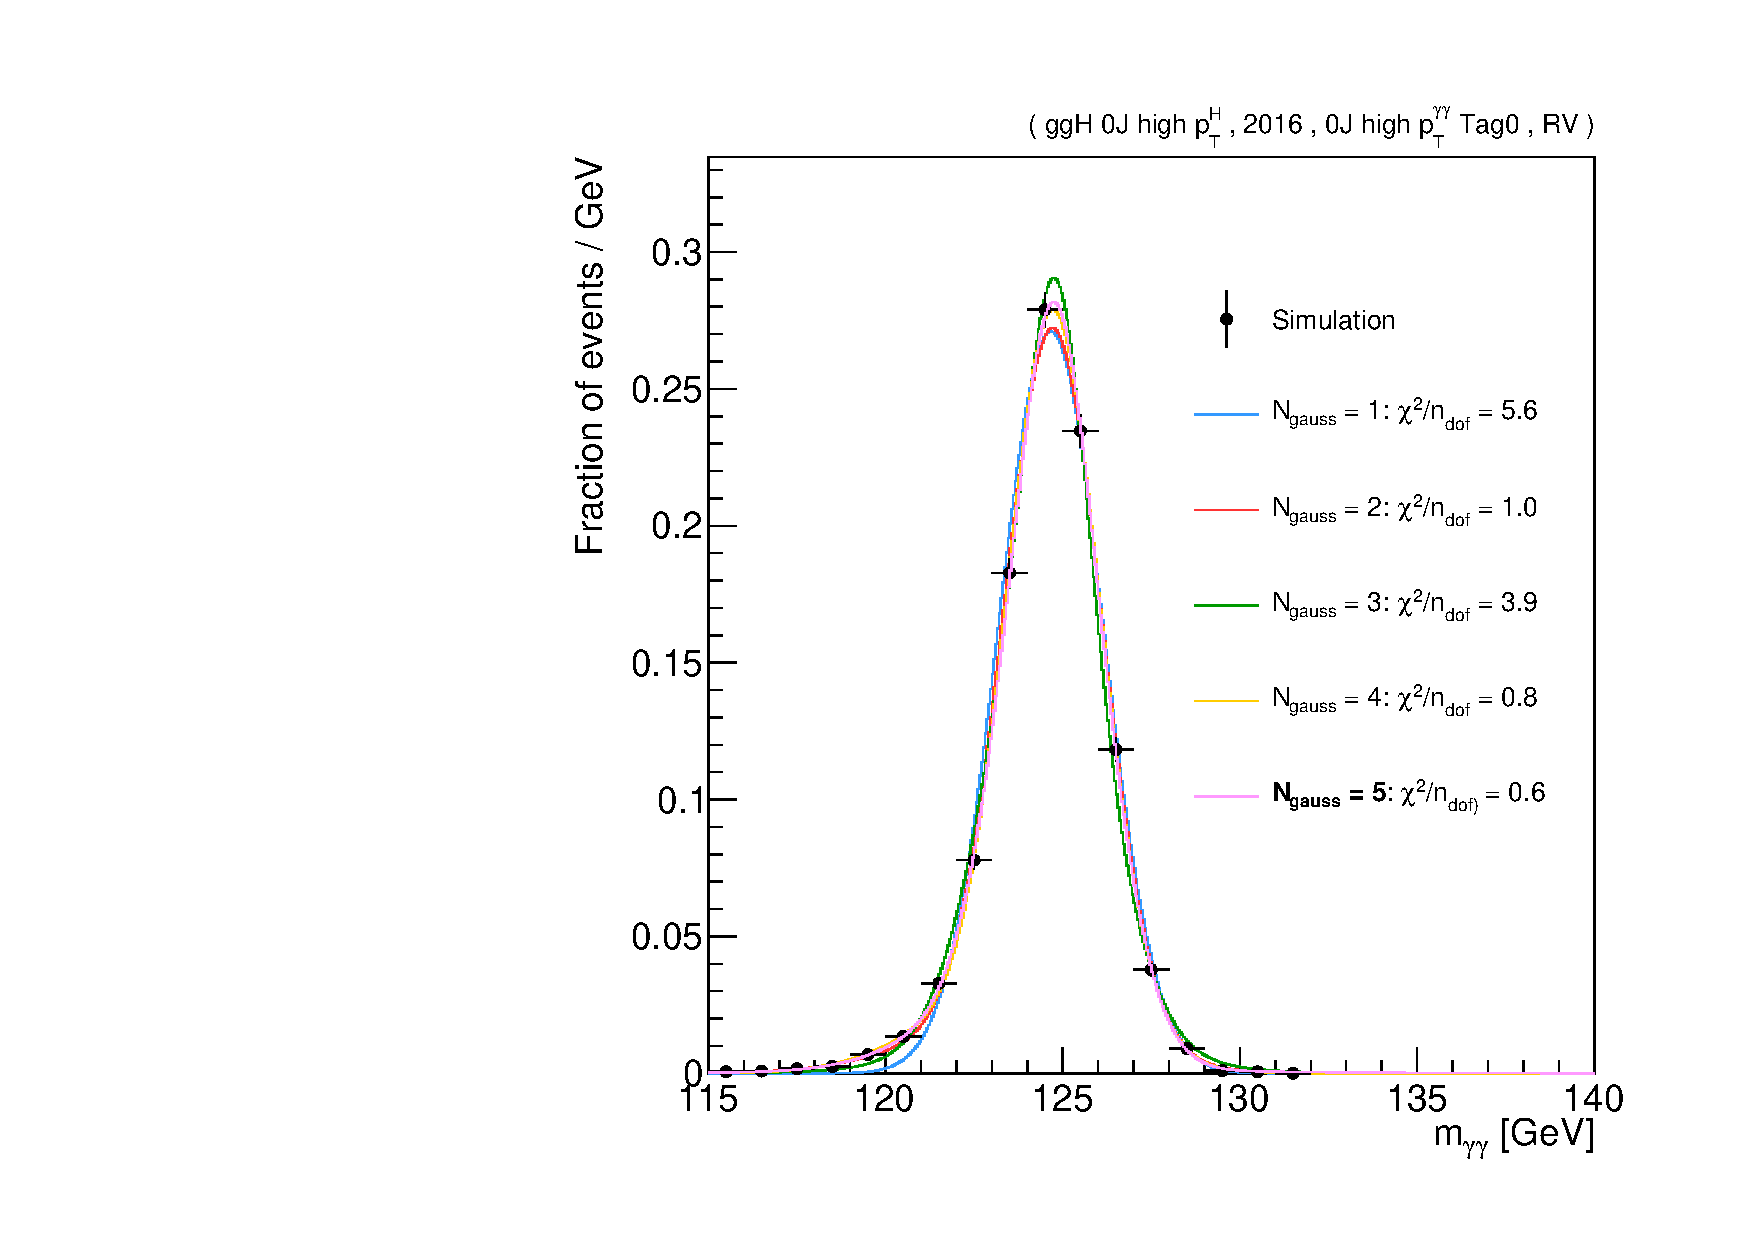
\includegraphics[width=.49\textwidth]{Figures/hgg_stats/fTest_RECO_0J_PTH_GT10_Tag0_GG2H_0J_PTH_GT10_RV.pdf}
  \hfill
  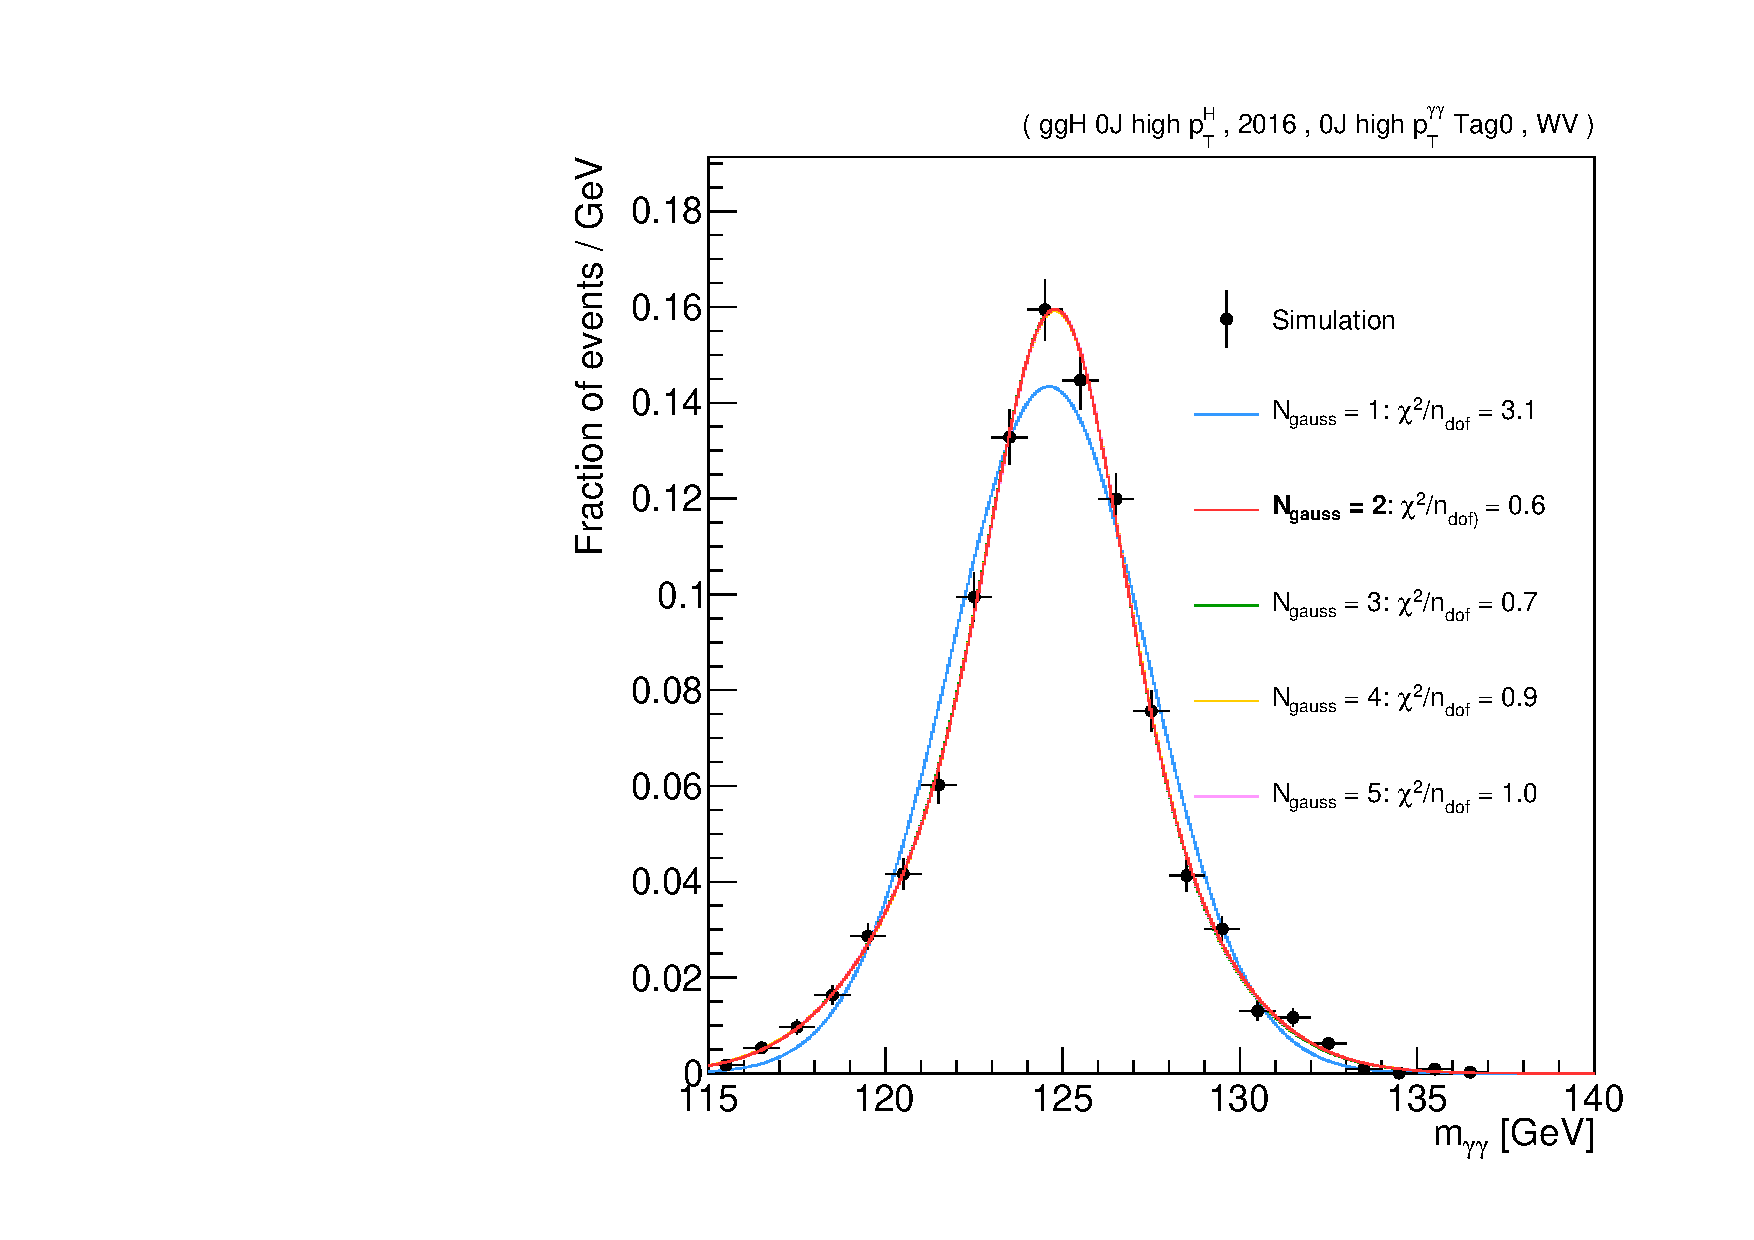
\includegraphics[width=.49\textwidth]{Figures/hgg_stats/fTest_RECO_0J_PTH_GT10_Tag0_GG2H_0J_PTH_GT10_WV.pdf}
  \caption[Signal modelling: number of Gaussians]
  {
    Different number of Gaussians
  }
  \label{fig:sigmodels_ftest}
\end{figure}

\begin{figure}
  \centering
  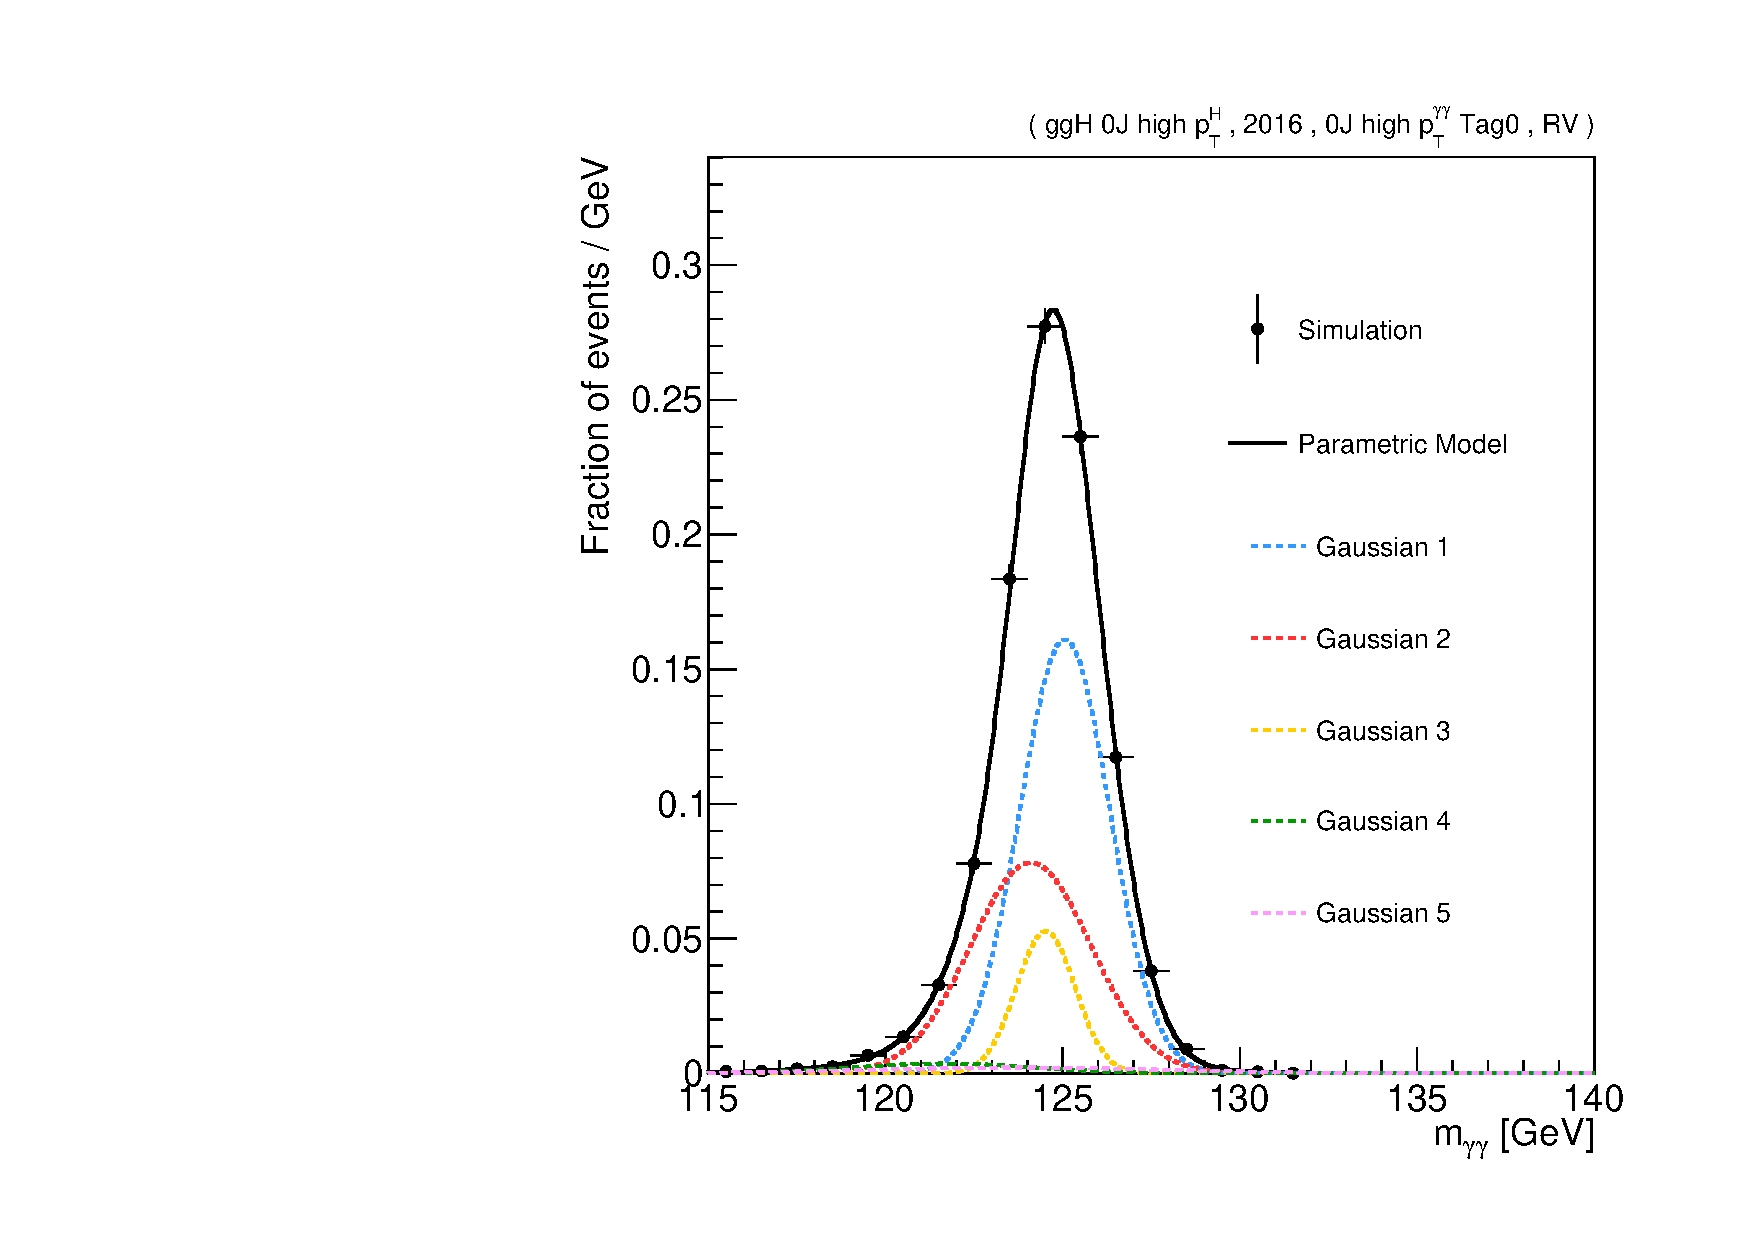
\includegraphics[width=.49\textwidth]{Figures/hgg_stats/RV_shape_pdf_components_GG2H_0J_PTH_GT10_RECO_0J_PTH_GT10_Tag0.pdf}
  \hfill
  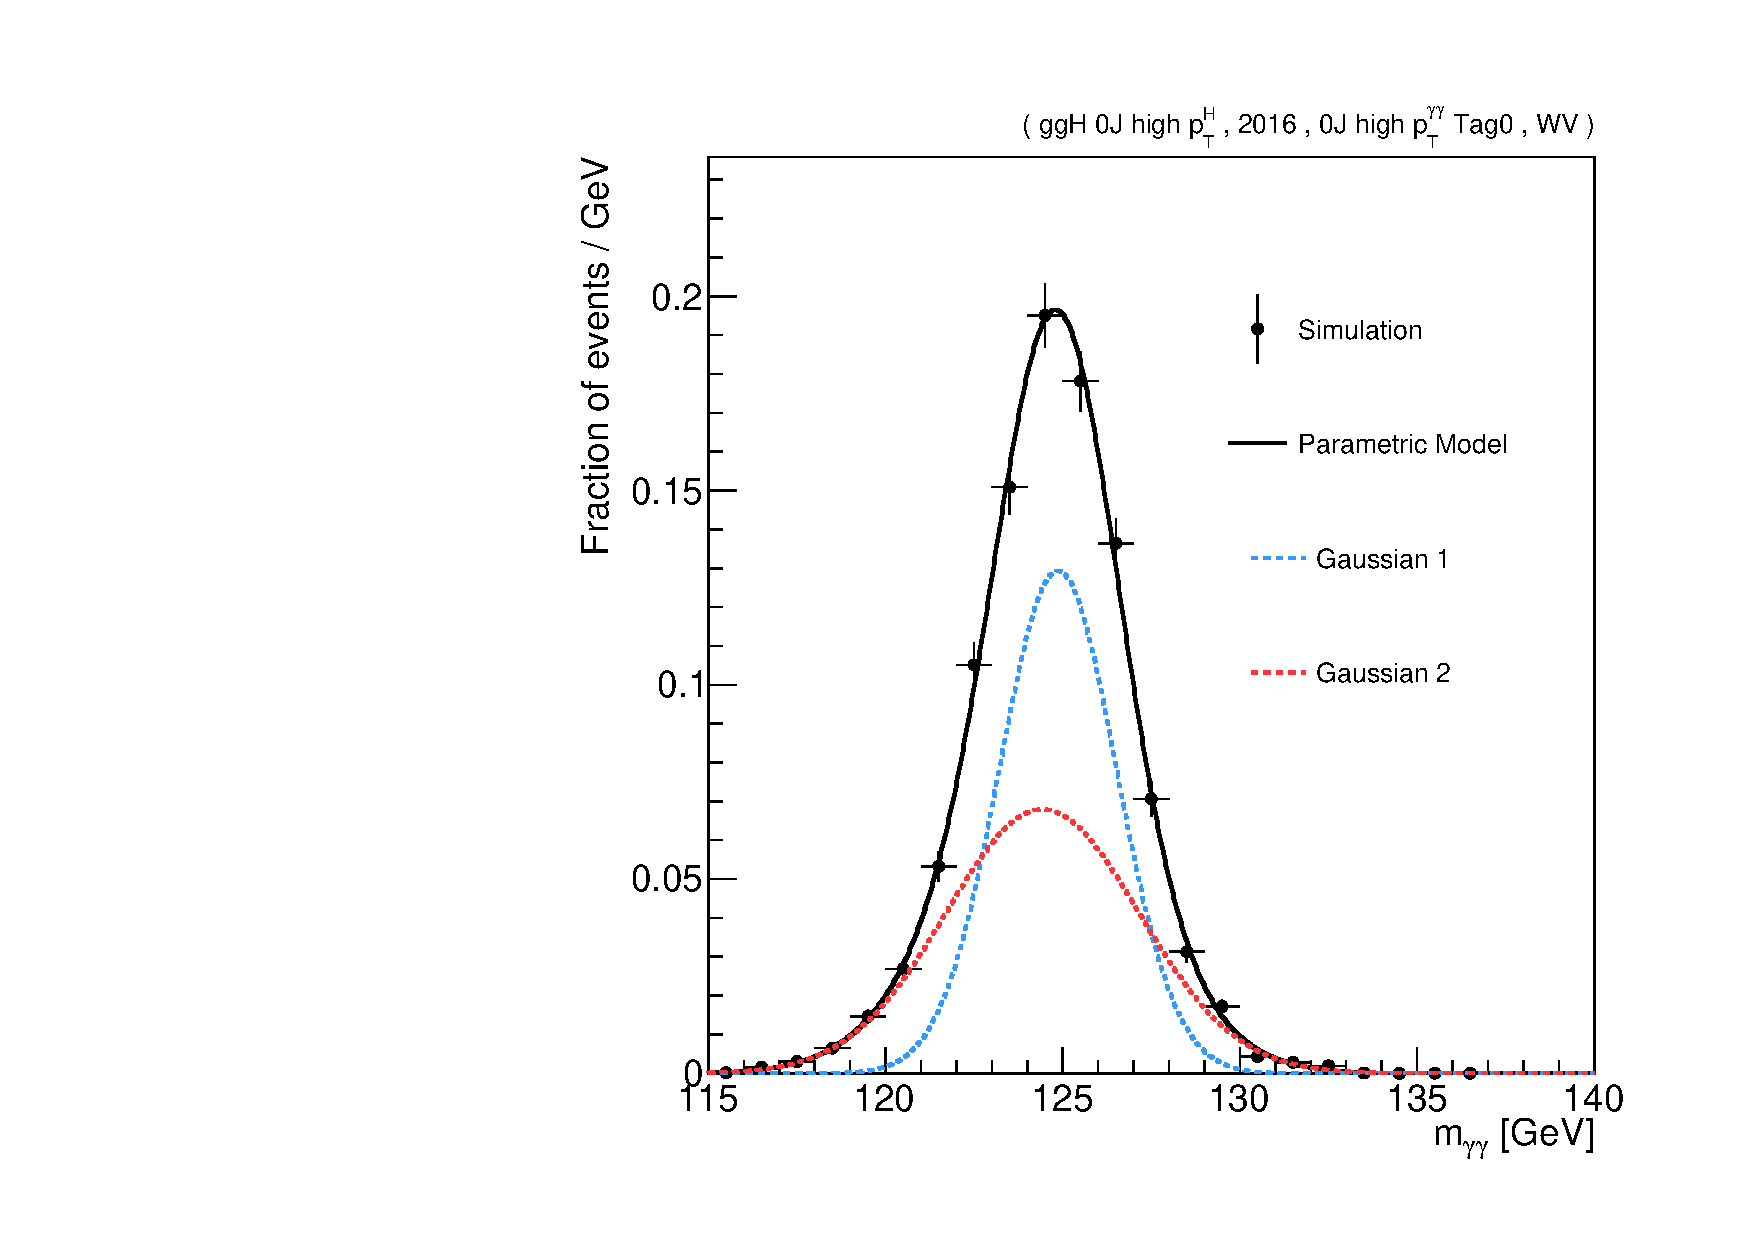
\includegraphics[width=.49\textwidth]{Figures/hgg_stats/WV_shape_pdf_components_GG2H_0J_PTH_GT10_RECO_0J_PTH_GT10_Tag0.pdf}
  \caption[Signal modelling: components]
  {
    Signal models for ggH 0J \pTH
  }
  \label{fig:signal_fitting}
\end{figure}

For a number of ($i$,$k$,$V$) combinations, particularly those corresponding to the far off-diagonal elements in Figure \ref{fig:purity_matrix}, there is an insufficient number of simulated events to accurately model the signal shape. In this case, the shape is replaced by that of the diagonal process, or in other words the STXS stage 1.2 bin with the highest yield in analysis category, $k$. This replacement is motivated by the fact that events in the same region of experimental phase space i.e subject to the same selection criteria, tend to have similar values of the diphoton mass resolution.

The signal models are normalised according to equation \ref{eq:signal_yield}. The SM predictions of the cross sections and the \Hgg branching ratio, evaluated at $m_H=125.38$~GeV, are taken from Ref.~\cite{deFlorian:2016spz}, and the fractional breakdowns into the respective STXS stage 1.2 bins are calculated directly from the MC samples. As mentioned above, the efficiency times acceptance terms, $\epsilon^{i,\gamma\gamma}_{k}$, are derived separately for each year. The values are calculated directly from MC simulation with $m_H$~=125.0~GeV, by dividing the yield of stage 1.2 bin, $i$, falling in category $k$, by the total yield of that bin. Again, this approach works under the assumption that the variation in $\epsilon^{i,\gamma\gamma}_{k}$ is negligible in going from $m_H=125.0$~GeV to 125.38~GeV. The 2018 $\epsilon^{i,\gamma\gamma}_{k}$ terms for a reduced set of stage 1.2 bins\footnote{In the analysis, the $\epsilon^{i,\gamma\gamma}_{k}$ terms are calculated for each individual STXS stage 1.2 bin. The reduced set of signal processes is used only for plotting purposes.} are shown in the matrix in Figure \ref{fig:ea_2016}. The bottom row, labelled as ``NO TAG", represents the fraction of events which do not enter any of the analysis categories. Equivalent matrices are shown for 2016 and 2017 MC in Appendix XXX.

\begin{figure}[hptb]
  \centering
  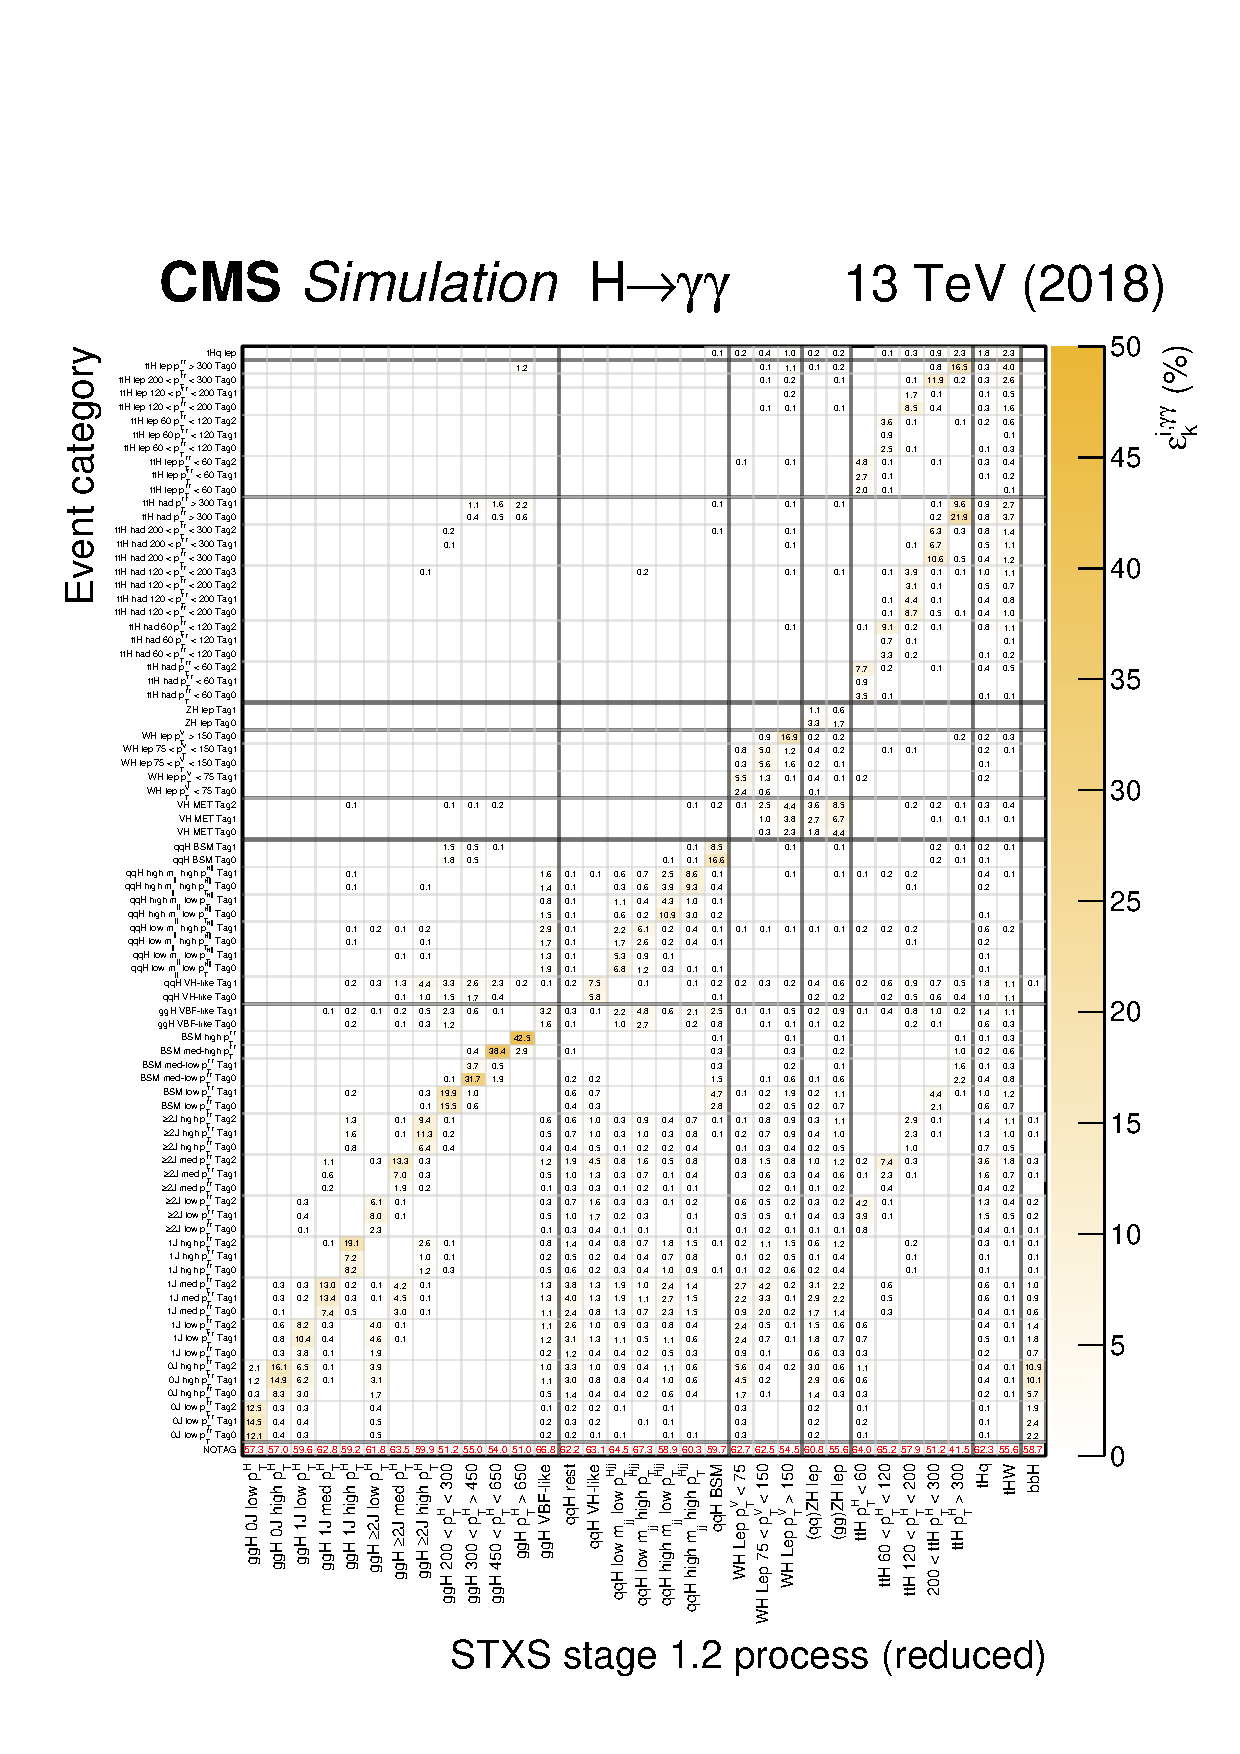
\includegraphics[width=1\textwidth]{Figures/hgg_stats/migrationMatrix_2018_thesis.pdf}
  \caption[Efficiency times acceptance matrix from 2016 simulation]
  {
    A matrix showing the $\epsilon^{i,\gamma\gamma}_{k}$ terms for a reduced set of STXS bins, derived from 2018 simulation. The numbers corresponds to the fraction of the total yield of STXS bin, $i$, landing in analysis category, $k$, expressed as a percentage. Each column therefore sums to 100\%. Entries with values less than 0.05\% are not shown. The bottom row indicates the fraction of events which do not enter a single analysis category. The column labelled as qqH rest includes the contributions from the qqH 0J, qqH 1J, qqH $m_{jj}<60$~GeV and the qqH $120<m_{jj}<350$~GeV STXS bins.
  }
  \label{fig:ea_2016}
\end{figure}

One can plot the per-category signal model by summing the individual models of each STXS stage 1.2 bin,
\begin{equation}
    \mathcal{S}_k = \sum_i \mathcal{S}^{i,\gamma\gamma}_k = \sum_i f_{RV} \cdot \mathcal{S}^{i,\gamma\gamma}_{k,RV} + (1-f_{RV}) \cdot\mathcal{S}^{i,\gamma\gamma}_{k,WV}.
\end{equation}
\noindent
Figure \ref{fig:sigmodels_category} shows the per-category signal models for the 0J high \ptH Tag0 and qqH VH-like Tag0 categories. The $\sigma_{\rm{eff}}$, defined as half of the smallest interval containing 68.3\% of the invariant mass distribution, is used to quantify the diphoton mass resolution. In the plots, the models are split into the contributions from each year, and the respective $\sigma_{\rm{eff}}$ values are displayed. In general, the detector performance, and therefore the diphoton mass resolution, worsen as a function of time due to radiation damage in the electromagnetic calorimeters. However, an extensive and thorough offline reconstruction program was developed specifically for the 2017 data, resulting in improved diphoton mass resolution and therefore smaller values of $\sigma_{\rm{eff}}$. Such offline reconstruction programs are planned for the 2016 and 2018 data in the future. 

\begin{figure}[hptb]
  \centering
  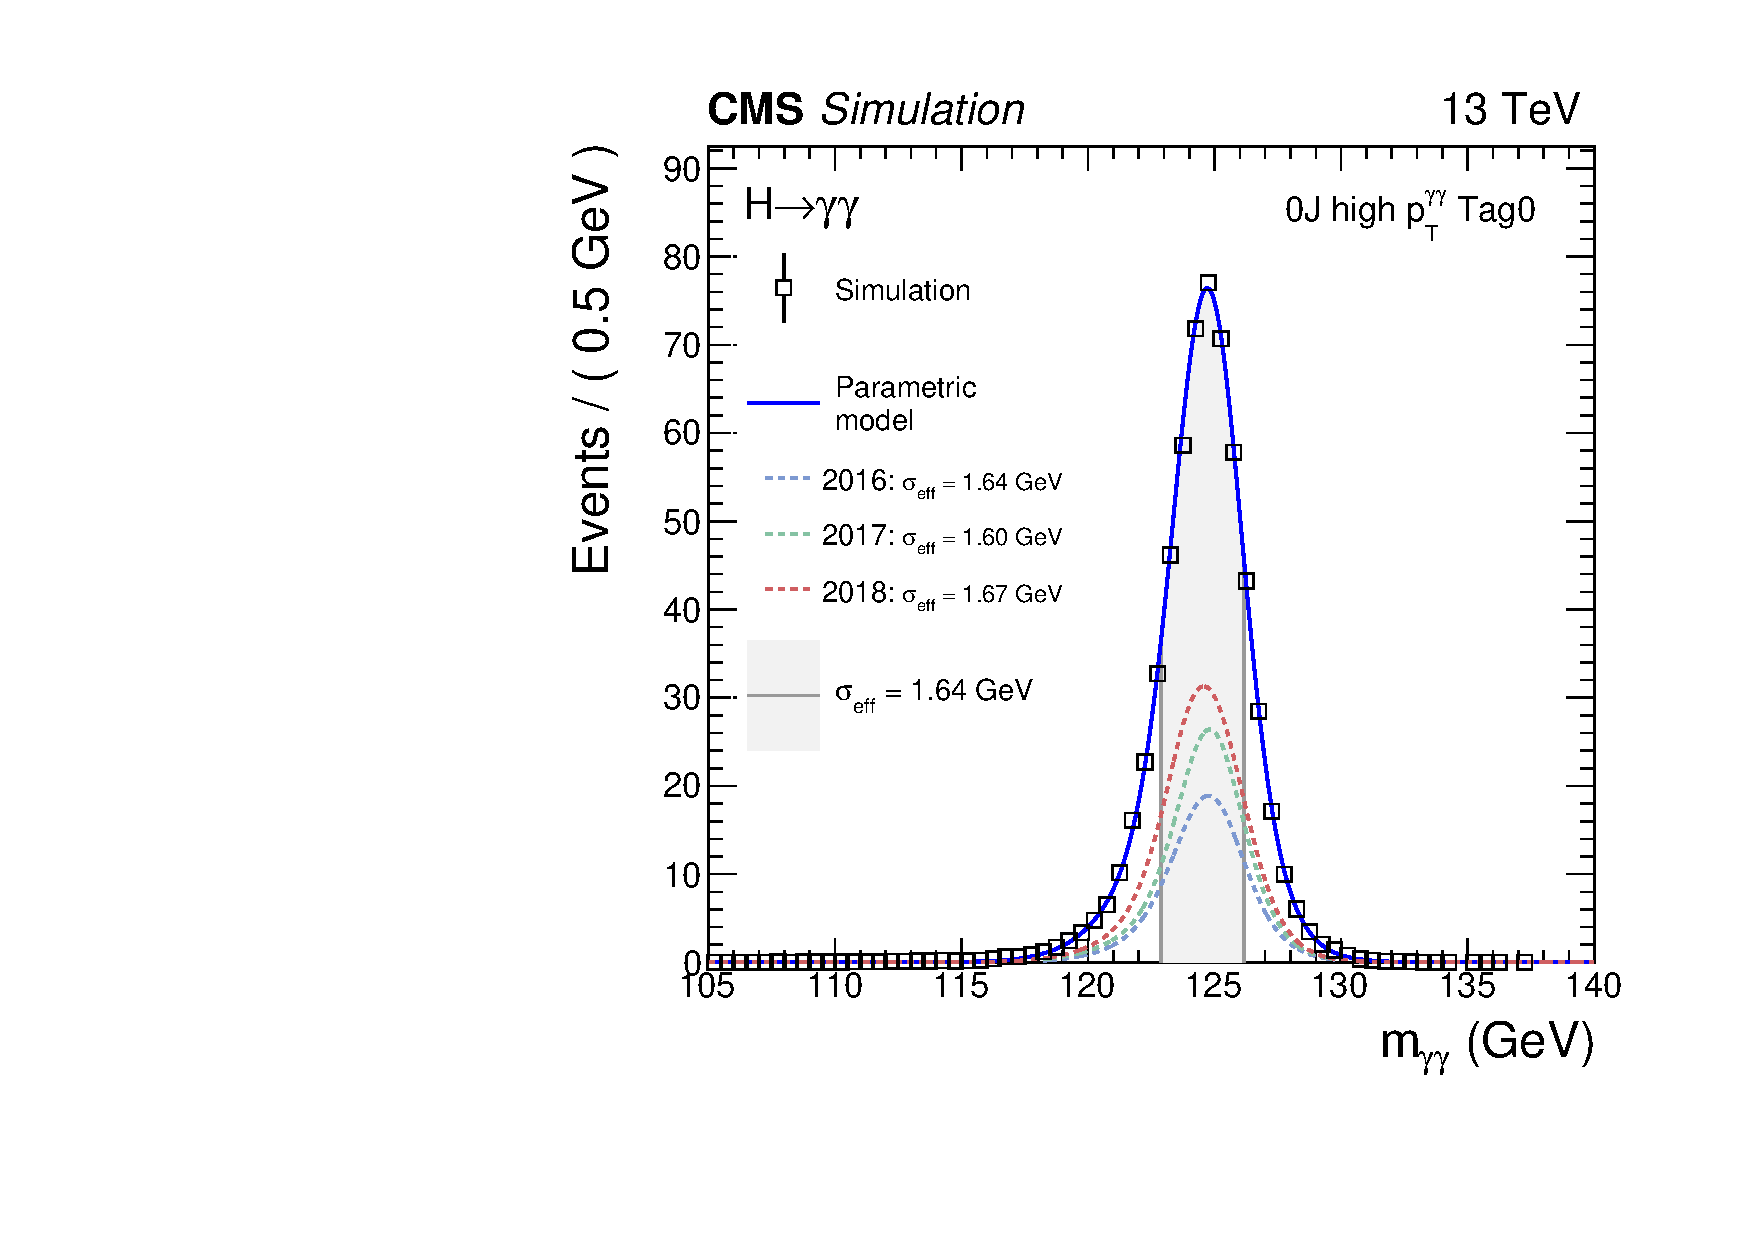
\includegraphics[width=.49\textwidth]{Figures/hgg_stats/smodel_RECO_0J_PTH_GT10_Tag0.pdf}
  \hfill
  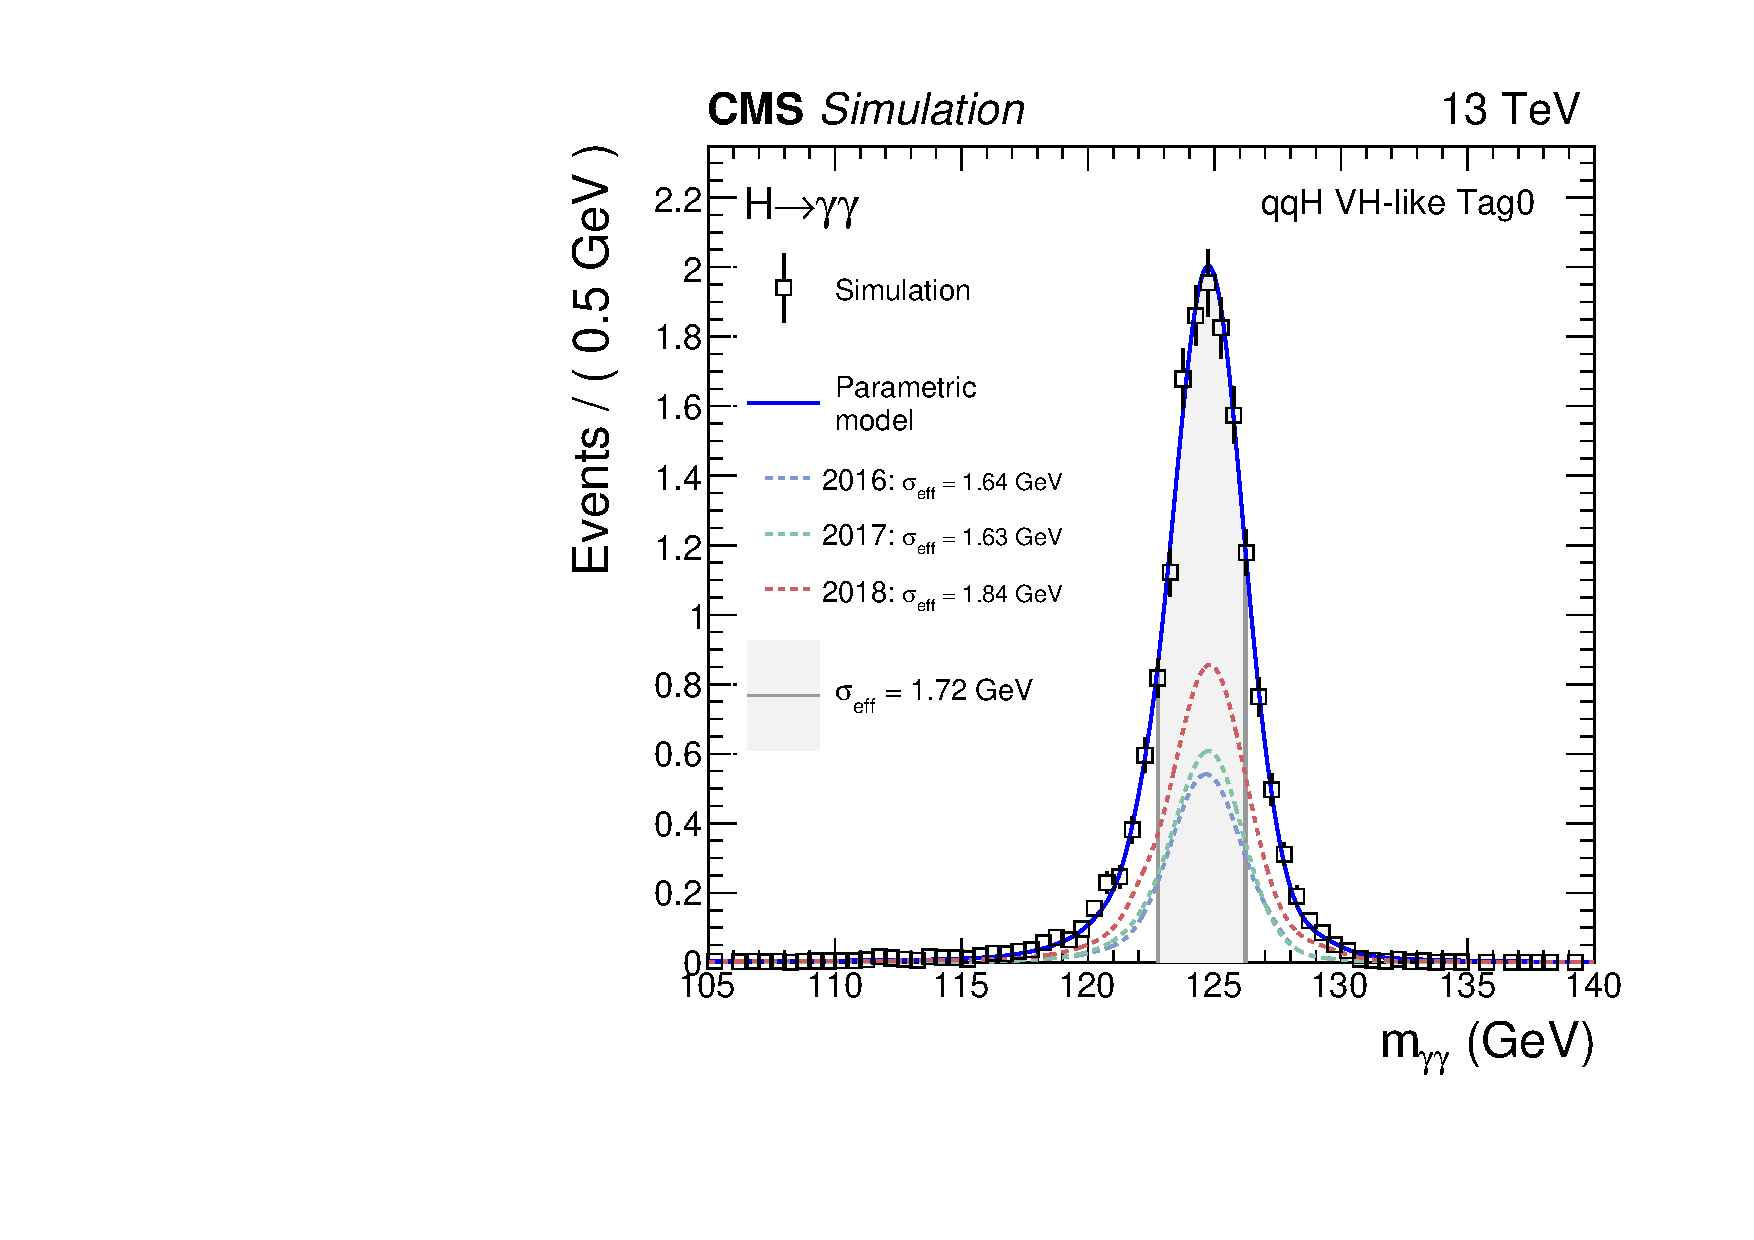
\includegraphics[width=.49\textwidth]{Figures/hgg_stats/smodel_RECO_VBFTOPO_VHHAD_Tag0.pdf}
  \caption[Signal models for the 0J low \ptH Tag0 and qqH VH-like Tag0 categories]
  {
    Add caption.
  }
  \label{fig:sigmodels_category}
\end{figure}

Going further, we can plot the sum of all per-category models to show the total signal model, $\mathcal{S}$. In Figure \ref{fig:sigmodels_weighted}, each per-category model is weighted in the sum according to the $F_{68} = S_{68}/(S_{68}+B_{68})$ values displayed in Tables \ref{tab:ggH_category_yields}--\ref{tab:top_category_yields}, such that the total signal yield remains constant. The explicit form of the weighted sum is shown in Equation \ref{eq:sigmodel_wsum}, where the index, $l$, runs over all analysis categories,

\begin{equation}\label{eq:sigmodel_wsum}
    \mathcal{S}^' = \sum_k w_k\,\mathcal{S}_k; \qquad w_k = (F^k_{68}) \times \frac{\sum_l S^l_{68}}{\sum_l F^l_{68} S^l_{68}}.
\end{equation}

\begin{figure}[hptb]
  \centering
  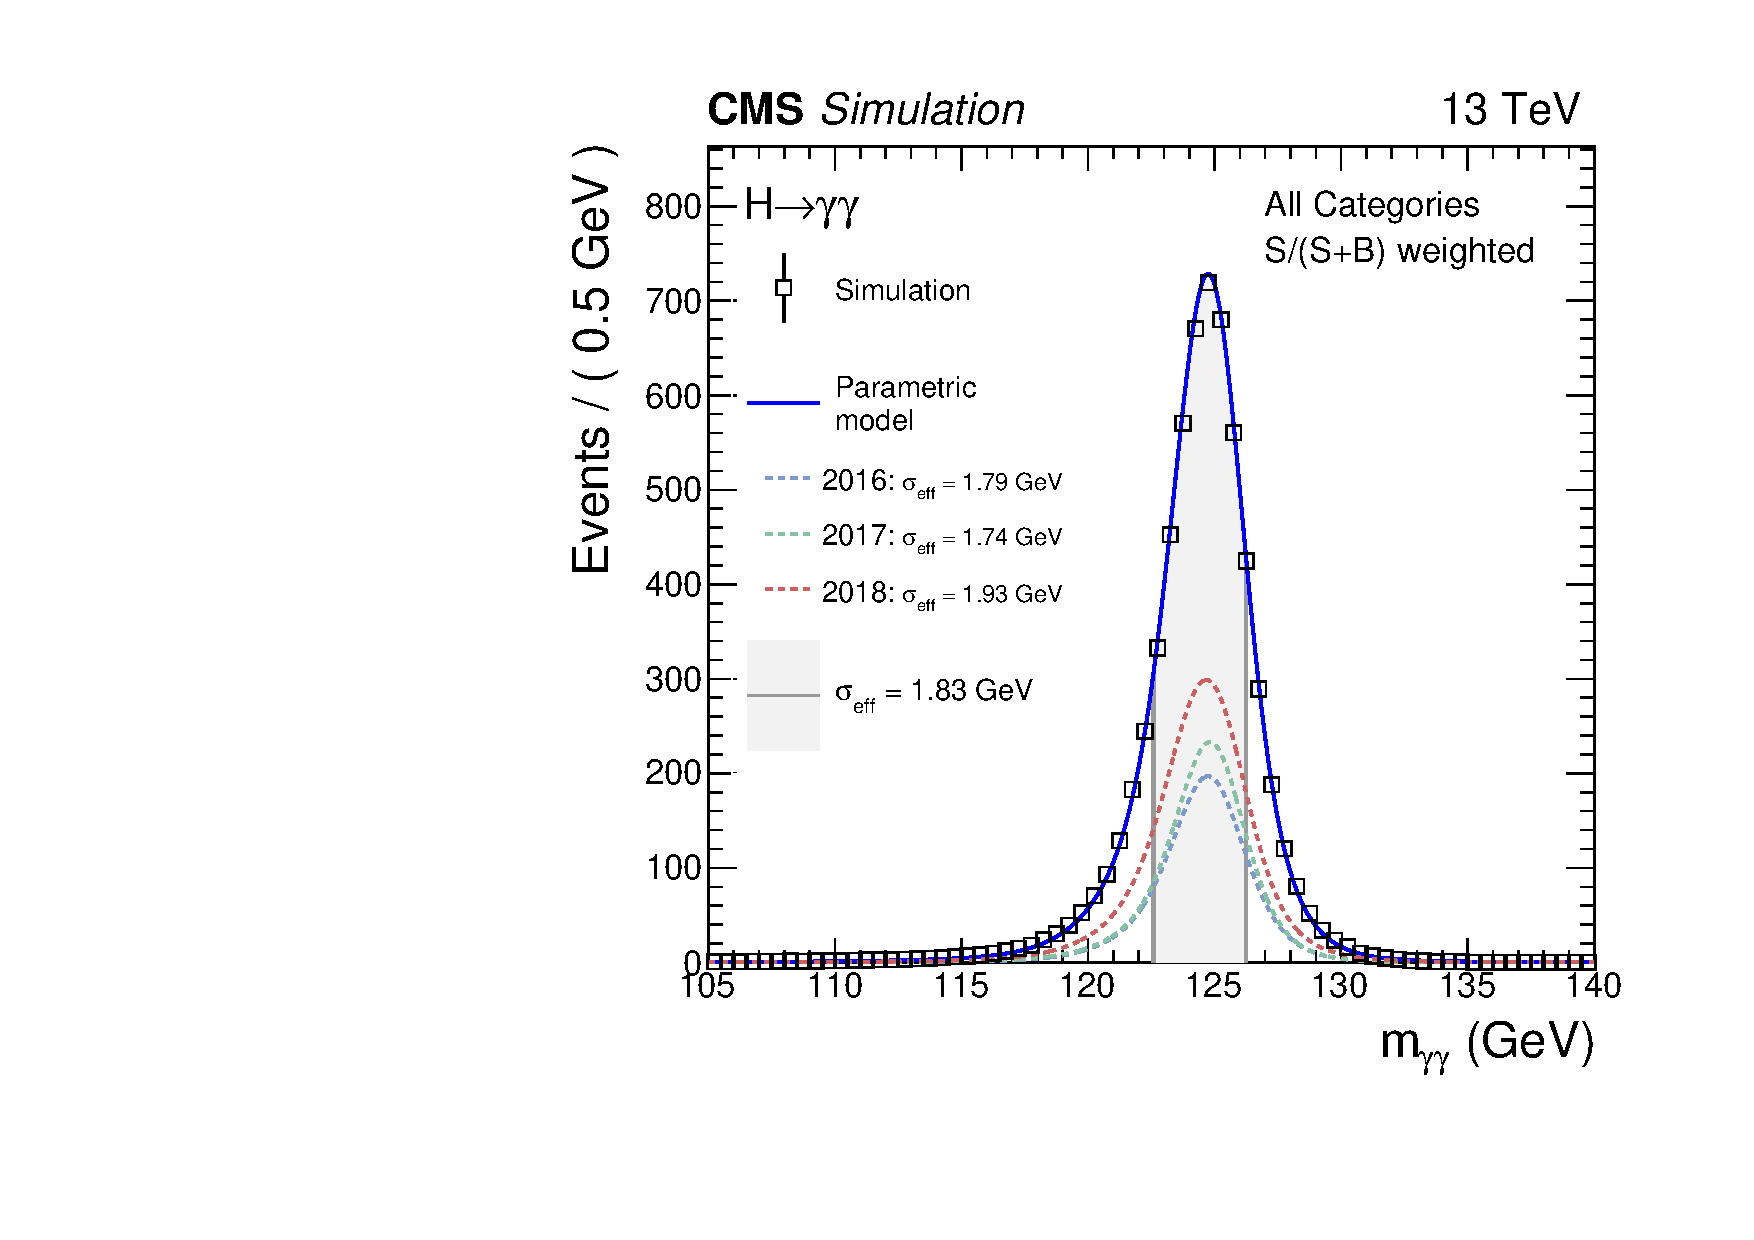
\includegraphics[width=.8\textwidth]{Figures/hgg_stats/smodel_all_weight.pdf}
  \caption[Weighted sum of all signal models]
  {
    Add caption.
  }
  \label{fig:sigmodels_weighted}
\end{figure}

\section{Background modelling}\label{sec:bkg_modeling}
Events entering the analysis categories that do not originate from Higgs boson production form a smoothly falling \mgg distribution, on top of which the signal peak resides. To derive the $B_{k,X}$ terms of equation \ref{eq:category_likelihood}, an analytic model is constructed in each analysis category to describe the distribution of background events. These models are extracted directly from data.

The underlying shape of the background distribution is not \textit{a priori} known, and therefore a number of functional forms must be considered. Ultimately, this analysis amounts to measuring a small Higgs boson signal sitting on top of a larger background. As a result, relatively small changes in the background model shape and thus the estimated background contribution under the signal peak, may incur a variation in the measured signal parameters of interest. This property of the analysis means that the uncertainty in the choice of background function must be accounted for.

\subsection{The effect of nuisance parameters on the likelihood}
Before introducing the background modelling technique in detail, it is worth taking time to understand the effect of nuisance parameters on the likelihood. When minimising the quantity $-2\ln{L}$, the nuisance parameters representing systematic uncertainties are profiled: their value is free to vary during the minimisation, in accordance with the specified constraint $\mathcal{C}$, but their final value is not of interest. The increased freedom in the fit means that for a given point in parameter space, $\vec{\alpha}$, a configuration of the nuisance parameters can be found, $\vec{\theta}_{\vec{\alpha}}$, which increases the likelihood, $L$, or equivalently decreases the value of $-2\ln{L}$. This manifests as a widening of the $q(\vec{\alpha})$ curve, and therefore an increase of the uncertainty in the fitted parameters of interest.

The contribution to the total uncertainty from an individual nuisance parameter, $\theta$, is realised by fixing the nuisance parameter to it's best-fit value, $\hat{\theta}$, in the fit. The width of the resulting $q(\vec{\alpha})$ curve represents the total uncertainty without the effect of $\theta$, and therefore will be narrower than curve in which $\theta$ is profiled. This is such that the quadrature-difference in the curve widths equates to the contribution to the uncertainty from $\theta$. In this analysis, we use this technique to evaluate the \textit{impact} of each uncertainty source on the parameters of interest. In addition, by fixing groups of nuisance parameters to their best-fit values, it is possible to decompose the total uncertainty into contributions from theoretical sources ($\vec{\theta}^{\,\rm{th}}_{s}$, $\vec{\theta}^{\,\epsilon,{\rm{th}}}_{s}$), experimental sources ($\vec{\theta}^{\,\epsilon,{\rm{exp}}}_{s}$, $\vec{\theta}^{\,\rm{shape}}_{s}$, $\vec{\theta}^{\,\rm{lumi}}_{s}$), and the statistical component\footnote{Here, the background model nuisance parameters, $\vec{\theta}^{\,\rm{shape}}_{b}$, $\vec{\theta}^{\,\rm{discrete}}_{b}$, are grouped with the statistical uncertainty.}. 

Figure \ref{fig:nuisance_illustration} illustrates a different approach to the same conclusion. The blue curve represents a fit in which the nuisance parameter in question, $\theta$, is fixed to it's best fit value. By fixing $\theta$ to different values, it is possible to build up a series of likelihood curves, shown by the dashed red lines, with minima shifted from the unconditional best-fit point. The minimum envelope of these likelihood curves, shown by the dashed green line, can be used to approximate the contribution to the uncertainty from $\theta$. In the limit of infinitesimally small steps in $\theta$, the envelope converges to the fully profiled likelihood curve (black line).

\begin{figure}[hptb]
  \centering
  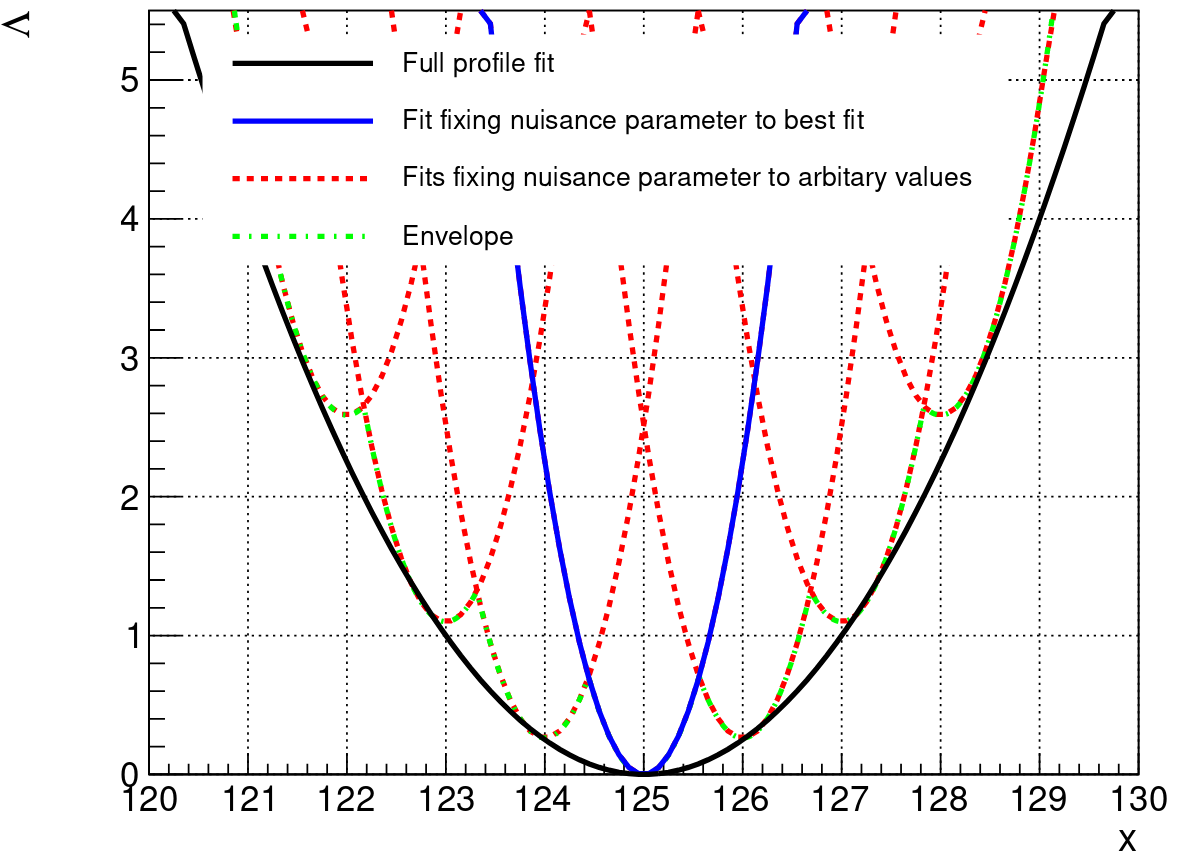
\includegraphics[width=.8\textwidth]{Figures/hgg_stats/nuisance_illustration.png}
  \caption[Constructing the envelope]
  {
    Add caption.
  }
  \label{fig:nuisance_illustration}
\end{figure}

\subsection{Discrete profiling method}
The example described above was introduced in the context of a continuous nuisance parameter. This same approach of building the envelope can be extended to the discrete case, where the nuisance parameter is limited to discrete values, albeit provided there is sufficient freedom in the allowed values to provide good coverage of the uncertainty.

In this analysis, the so-called \textit{discrete profiling method} is applied to model the uncertainty in the choice of background function~\cite{Dauncey:2014xga}. A number of candidate functions are considered to fit the background in each category, and a discrete nuisance parameter is introduced to label the choice of function. In theory, the complete set of all analytic functions should be considered to obtain the exact uncertainty; in practice it is sufficient to consider a subset of functions which provide a reasonable fit to data. This keeps the computing time required for the full minimisation to a tolerable level. By allowing the value of the discrete nuisance, and thus the functional form of the background to vary, an envelope of likelihoods is constructed (as in Figure \ref{fig:}) which successfully approximates the uncertainty in the choice of background function.

\begin{table}[htb]
    \caption[Function families considered in the discrete profiling method]{Blah}
    \label{tab:photon_preselection}
    \vspace{.5cm}
    \centering
    \footnotesize
    \renewcommand{\arraystretch}{1}
    \begin{tabular}{m{0.35\textwidth}|p{0.55\textwidth}}
       Sum of exponentials & 
       \begin{equation*}
           f_N(x) = \sum^N_{i=0} p_{2i}\,{\rm{exp}}\big( p_{2i+1}x\big)
       \end{equation*} \\ \hline
       Sum of power law functions & 
       \begin{equation*}
           f_N(x) = \sum^N_{i=0} p_{2i}x^{-p_{2i+1}}
       \end{equation*} \\ \hline
       Bernstein polynomials & 
       \begin{equation*}
           f_N(x) = \sum^N_{i=0} p_i {N \choose i}x^i(1-x)^{N-i}
       \end{equation*} \\ \hline
       Laurent series &
       \begin{equation*}
           f_N(x) = \sum^N_{i=0} p_i x^{-4+g(i)}; \qquad g(i) = \sum^i_{j=0} (-1)^jj
       \end{equation*} \\      
    \end{tabular}
\end{table}

The different families of functions considered are listed in Table~\ref{tab:discrete_functions}. For each family, the form is shown for order, $N$, uniquely described by parameters: $p_0$, $p_1$, ..., $p_N$. The following procedure is used to determine the final set of candidate functions for a given analysis category, $\mathcal{F}^k$:
\begin{itemize}
    \item A background-only fit is performed to the \mgg distribution in data, using the lowest-order function in a given family. This is performed by minimising the value of $-2\ln{L}_b$, allowing the normalisation and shape parameters of the function to vary, where the subscript $b$ has been added to indicate this is a background-only fit. A penalty term, $P$, is added to $-2\ln{L}_b$, equal to the number of parameters in the function. This prevents functions with arbitrarily high freedom being chosen. The process is repeated, incrementally raising the order, until a minimum goodness-of-fit criteria is reached. All orders below are not considered in $\mathcal{F}^k$ as they do not fit the data well.
    
    \item For all subsequent orders, an F-test is performed to decide if the improvement in fit quality warrants the increase in function complexity~\cite{}. Using the same procedure, the $-2\ln{L}_b+P$ value is determined for the next-highest order function in the family. Given a large enough sample size, the difference in $-2\ln{L}_b+P$ values for successive orders, $\Delta$, is distributed according to the $\chi^2$ distribution with $m$ degrees of freedom, where $m$ is the difference in the number of parameters between the two orders. A $p$-value is calculated as,
    
    \begin{equation}
        p = {\rm{Prob}}\Big(\Delta<\,\Delta_{\rm{obs}}\,\Big|\,\chi^2(m)\Big),
    \end{equation}
    \noindent
    where $\Delta_{\rm{obs}}$ is the observed value in data. If the $p$-value is less than 0.05 then the improvement in fit quality is deemed worthwhile, and the higher-order function is added to $\mathcal{F}^k$. This step is repeated for successive orders until the calculated $p$-value is larger than 0.05. In this scenario, the higher-order function is deemed to be unnecessarily complex given the data and the procedure terminates.

    \item This process is repeated for each of the four families listed in Table \ref{tab:discrete_functions}, where each order passing the above selection procedure enters $\mathcal{F}^k$.
\end{itemize}

The set of candidate functions, $\mathcal{F}^k$, are shown for the XX and YY analysis categories in Figure \ref{fig}. Clearly, the different functional forms provide a different background estimate when integrating under the signal peak. This sometimes large variation in the background estimate gives rise to an uncertainty in the fitted signal parameters of interest, originating from the lack of knowledge of the true background functional form.

\begin{figure}[hptb]
  \centering
  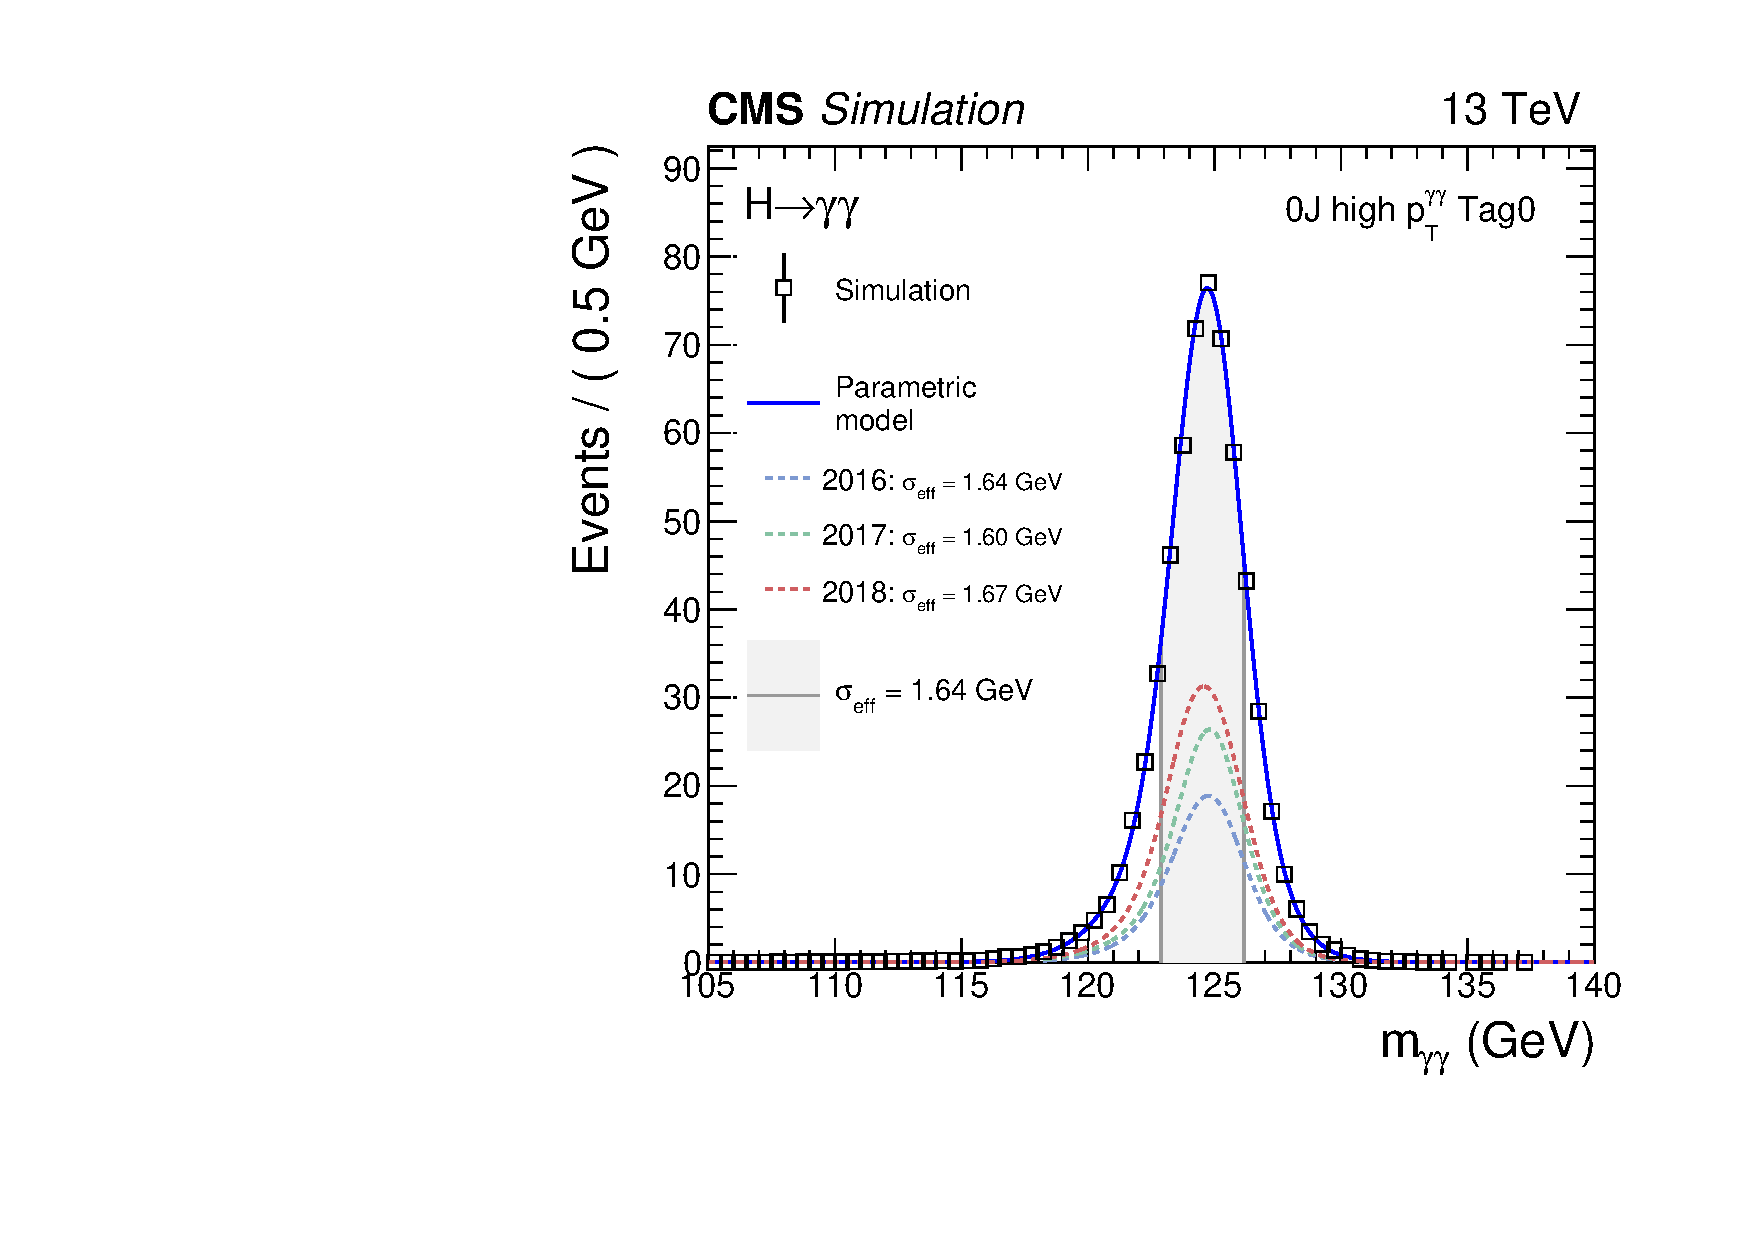
\includegraphics[width=.49\textwidth]{Figures/hgg_stats/smodel_RECO_0J_PTH_GT10_Tag0.pdf}
  \hfill
  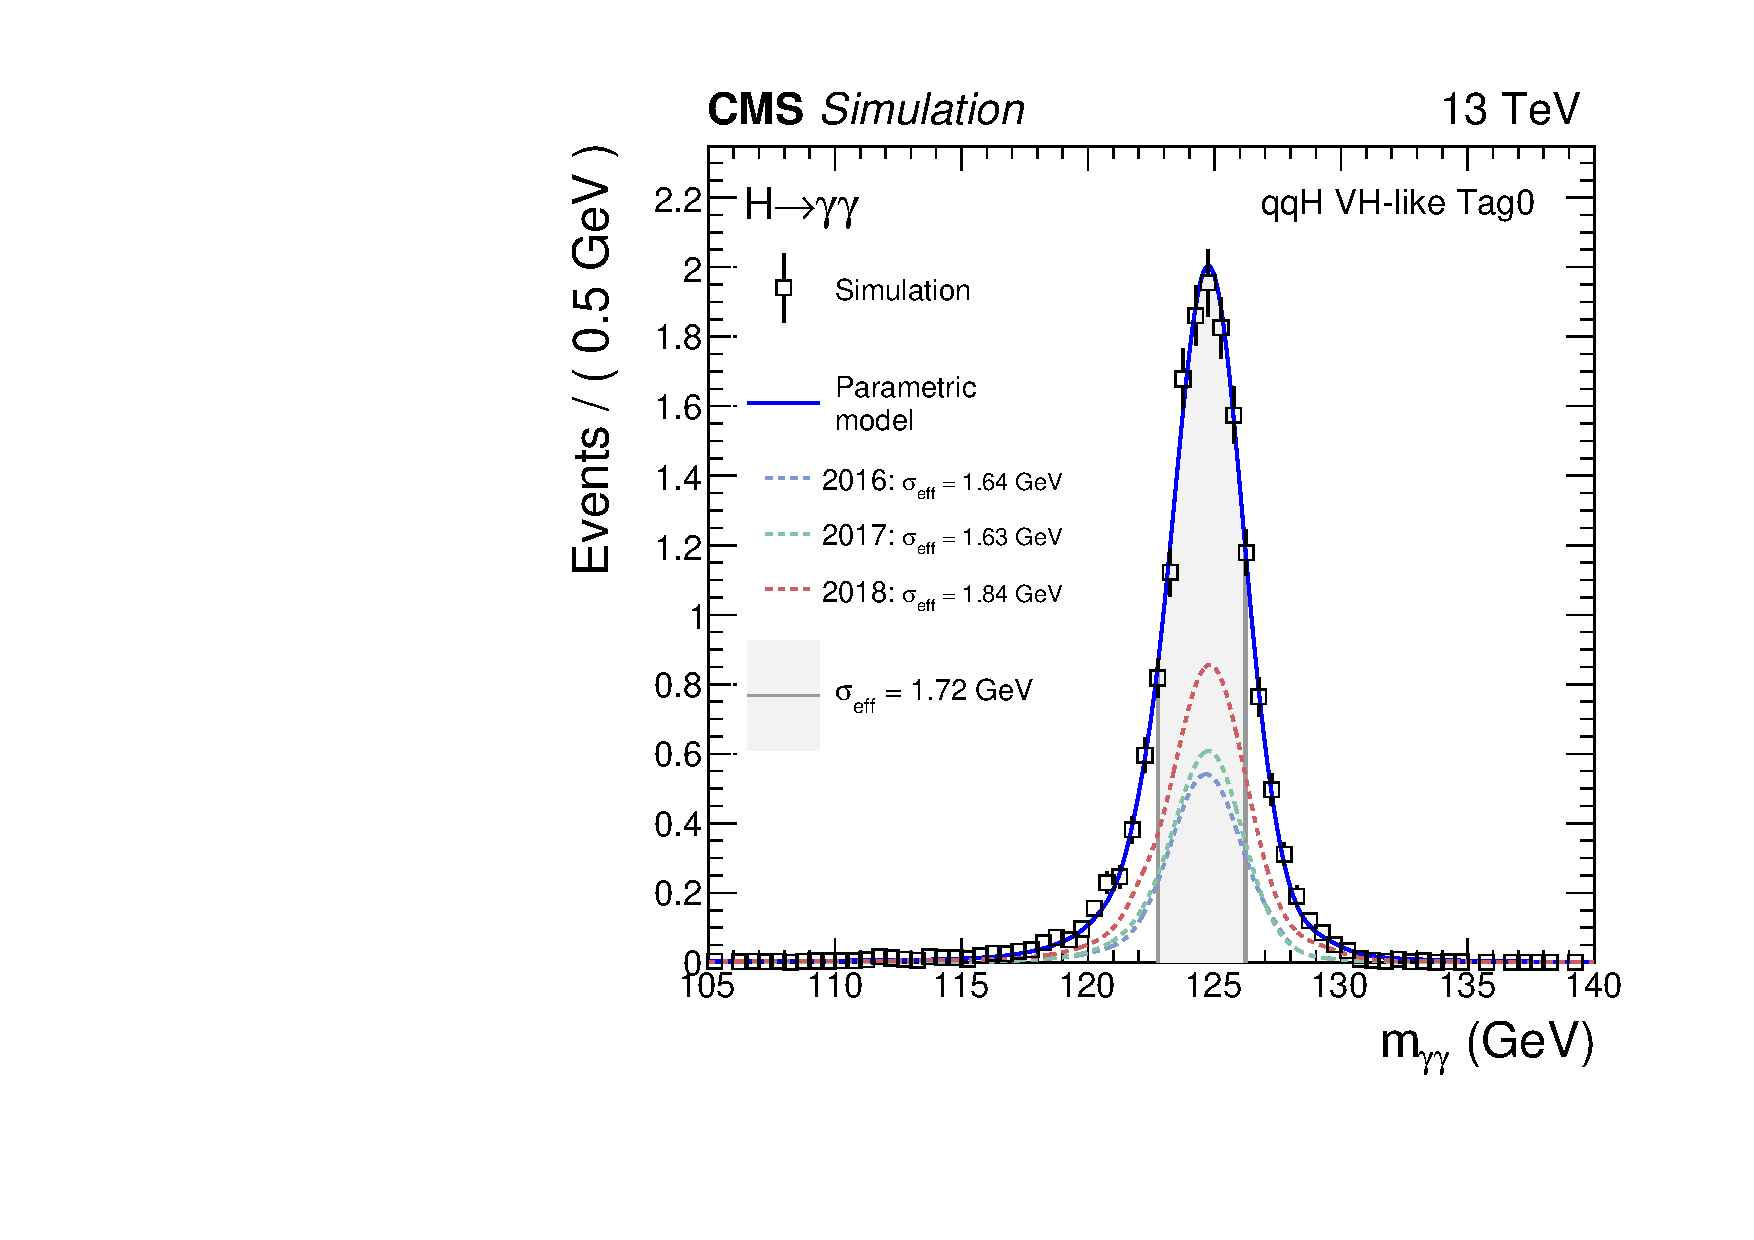
\includegraphics[width=.49\textwidth]{Figures/hgg_stats/smodel_RECO_VBFTOPO_VHHAD_Tag0.pdf}
  \caption[Signal models for the 0J low \ptH Tag0 and qqH VH-like Tag0 categories]
  {
    Add caption.
  }
  \label{fig:sigmodels_category}
\end{figure}

In the final results extraction (see section \ref{sec:results_extraction}), both the discrete nuisance parameters describing the choice of background functions ($\vec{\theta}^{\,\rm{discrete}}_{b}$), and the parameters of the functions themselves ($\vec{\theta}^{\,\rm{shape}}_{b} \equiv p_0,...,p_N$) are free to vary. In accordance with the procedure described above, a penalty term is added to the value of $-2\ln{L}$ equal to the number of parameters in the chosen function, thus penalizing functions with high complexity. Further details concerning the discrete profiling method are provided in Ref.~\cite{Dauncey:2014xga}. This includes a series of tests to show the method provides good coverage of the uncertainty in the choice of background function and leads to unbiased estimates of the parameters of interest.

\section{Systematic uncertainties}\label{sec:systematics}
A systematic uncertainty is included in the analysis to account for the minor differences between photon and electron. Signal shape etc. Vertex assignment.
\subsection{Theoretical uncertainties}
Acceptance and normalisation. Complication when merging bins.

\subsection{Experimental uncertainties}
Signal shape systematics: how are they calculated. Correlated with effect on rate. Plot showing the maximum effect (are nuisance params pulled to 1sigma).


\subsection{Correlation schemes}